\chapter{Задание исходной модели}
\label{cha:code-gen}

Хотя исходными данными для построения модели Крипке служит набор автоматов Мили
(см.~\ref{cha:model-checking}), задавать модель непосредственно в таком виде неудобно:
желательно представлять ее в виде некоторой текстовой нотации.

\section{Выбор используемой нотации}
\label{sec:notation-choice}

В качестве нотации, используемой для задания модели, выбрано подмножество языка PROMELA,
описанного в \ref{sec:promela} и используемого верификатором SPIN. Это позволяет
использовать модели, созданные для SPIN, с минимальными изменениями. 

Следующие возможности PROMELA не реализованы:

\begin{enumerate}
\item Возможность создания новых процессов (т.е. все процессы должны быть активны изначально);
\item пользовательские типы данных (структуры и перечисления);
\item синхронные каналы (т.е. каналы нулевого размера, которые представляют собой <<точки
  рандеву>> между двумя процессами); поддерживаются асинхронные каналы ненулевого размера
  (за один переход возможна только одна операция с таким каналом -- запись одним процессом
  либо чтение другим);
\item возможность обращаться к явным и скрытым (IP) переменным других процессов.
\end{enumerate}

\section{Предобработка модели}
\label{sec:idef0-codegen}

Основное время при генерации состояний уходит на составление множества $Next(s)$ для
текущего состояний $s$. Оно заключается в вычислении условий выполнимости текущих
инструкций всех процессов, присутствующих в $s$ (отсюда мы получаем множество
незаблокированных процессов $P_{ready}(s)$), после чего для каждого процесса $P$ из
$P_{ready}(s)$ генерируется новое состояние, получающееся в результате выполнения его
текущей инструкции (номер которой хранится в $IP_P$).

Для достижения большей производительности генерация состояний осуществляется кодом на
языке~C, который, в свою очередь, генерируется из описания модели.

Функциональная модель всего процесса изображена на рис.~\ref{fig:idef0-codegen}. Исходное
описание модели считывается парсером и переводится во внутреннее представление в виде
графа команд и условий их выполнимости.

\begin{figure}[ht]
  \centering
  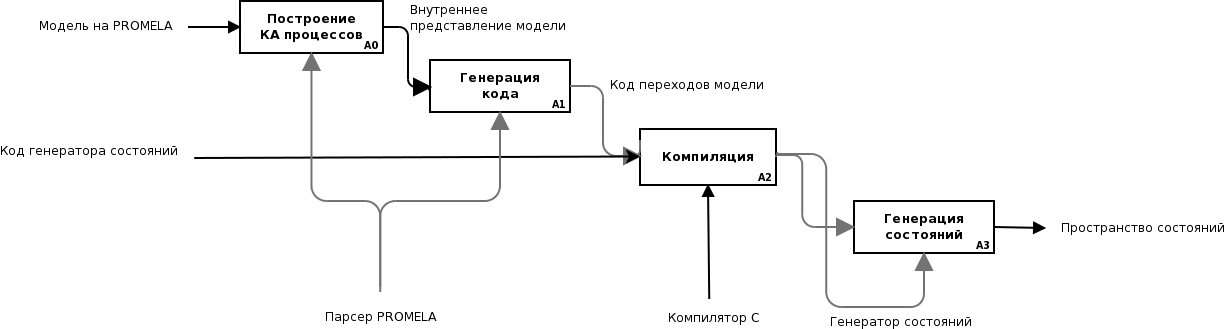
\includegraphics[width=1\textwidth]{../graphics/idef0-codegen}  
  \caption{Схема процесса верификации}
\label{fig:idef0-codegen}
\end{figure}

Генерируемый код на~C проверяет условия выполнимости текущих инструкций всех процессов и,
в случае выполнимости процесса $P$, создает новое состояние, являющееся копией текущего, и
модифирует его в соответствии с текущей инструкцией $P$.

Таким образом, генерируются следующие части кода:

\begin{itemize}
\item проверка выполнимости процессов данного состояний;
\item модификация состояния в соответствии с текущей инструкцией данного процесса;
\item вспомогательный код (отладочная печать состояния и т.п.).
\end{itemize}

Полученный код компилируется и компонуется вместе вместе с программой-<<драйвером>>
(осуществляющей выполнение не зависящих от конкретной модели операций: хэширование и
хранение состояний, передача по сети и~т.д.). Программа-<<драйвер>> делает вызовы функций
сгенерированного кода для вычисления $Next(s)$.

<<Драйверов>> имеется два: 

\begin{itemize}
\item последовательный, использованный в \ref{cha:paremu-test} для имитации параллельного
  выполнения с целью оценки распредления состояний;
\item описанный в \ref{cha:communication} параллельный на MPI.
\end{itemize}

\section{Парсинг описания модели и генерация кода}
\label{sec:promela-parser}

Парсер описания модели и генератор кода написан на языке Python. В качестве парсера
используется штатный GLR-парсер \Code{Pyggy}. Диаграмма классов генератора показана на
рис.~\ref{fig:pmlparse-classes}.

\begin{figure}[ht]
  \centering
  \includegraphics[width=1\textwidth]{../graphics/pmlparse-classes}
  \caption{Диаграмма классов генератора кода}
  \label{fig:pmlparse-classes}
\end{figure}

\section{Представление состояния}
\label{sec:state-represent}

\begin{figure}[ht]
  \centering
  \includegraphics[width=0.7\textwidth]{../graphics/state-representation}  
  \caption{Представление состояний}
  \label{fig:state-repr}
\end{figure}

\section{Задание проверяемых утверждений}
\label{sec:assertions}


%%% Local Variables: 
%%% mode: latex
%%% TeX-master: "thesis"
%%% End: 
